\subsubsection{Caso d'uso UC10.2: Modifica API}
\label{UC10.2}

\begin{figure}[ht]
	\centering
	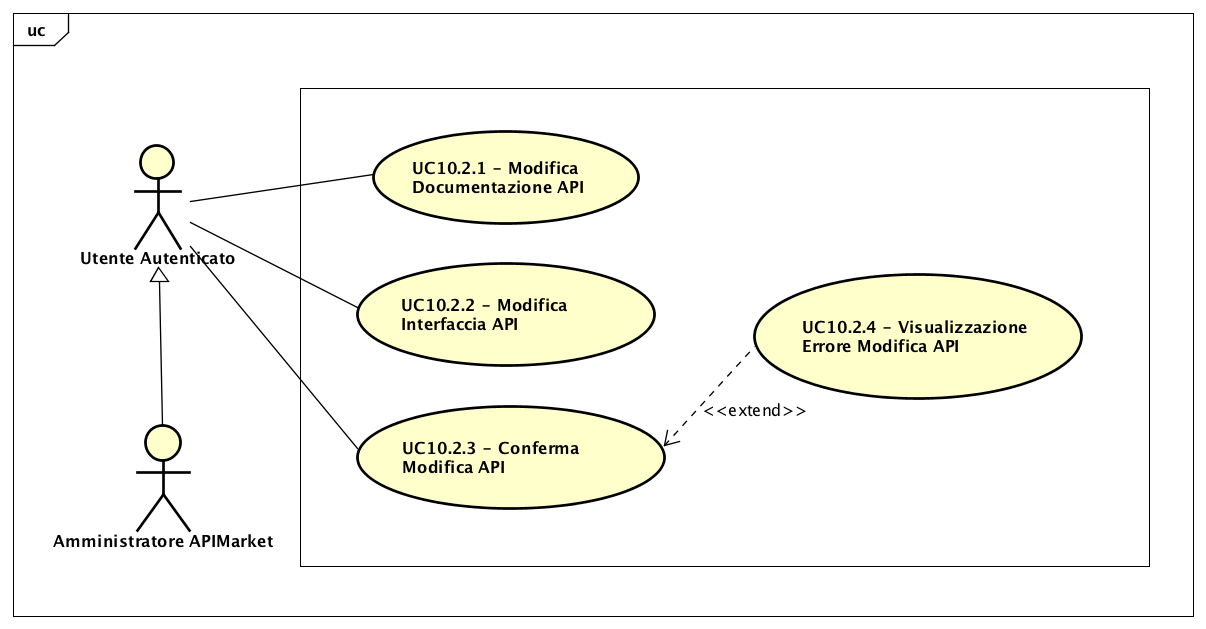
\includegraphics[scale=0.45]{UML/UC10_2.png}
	\caption{UC10.2: Modifica API}
\end{figure}

\renewcommand*{\arraystretch}{1.6}
\begin{longtable}{ l | p{11cm}}
	\hline
	\rowcolor{Gray}
	\multicolumn{2}{c}{UC10.2: Modifica API} \\
	\hline
	\textbf{Attori} &Utente Autenticato, Amministratore APIMarket \\
	\textbf{Descrizione} & l'attore modifica una propria API\\
	\textbf{Pre-Condizioni} & l'attore ha scelto di modificare una propria API\\
	\textbf{Post-Condizioni}&l'attore ha modificato una propria API oppure l'operazione è fallita\\
	\textbf{Scenario Principale} & \begin{enumerate*}[label=(\arabic*.),itemjoin={\newline}]
		\item l'attore può modificare la documentazione della propria API (UC10.2.1)
		\item l'attore può modificare l'interfaccia della propria API (UC10.2.2)
		\item l'attore può confermare le modifiche alla propria API (UC10.2.3)
	\end{enumerate*}\\
	\textbf{Scenari Alternativi} & \begin{enumerate*}[label=(\arabic*.),itemjoin={\newline}]
		\item l'attore può visualizzare l'errore di modifica API (UC10.2.4)
	\end{enumerate*}\\
\end{longtable}
